\thispagestyle{myheadings}
\chapter{関連研究}
 本章では本研究に関連するコンテンツについての研究や生体データを用いた研究,
重畳提示手法の研究,体験拡張研究の4つのテーマについて紹介する.本研究と比較し関連性や新規性を述べる.



\section{情報媒体における研究}
 コンテンツにはたくさんの種類がある.デジタルコンテンツにはYouTubeやNetflix,
アナログコンテンツには本や新聞紙などがある.
アナログコンテンツである本や新聞紙など紙で読む方がデジタルコンテンツで読むより記憶に残る研究がある\cite{books}.
スマートフォンの普及で本や新聞紙などを紙で読む機会が減った.そこで本研究のシステムを使えば,
アナログコンテンツにエフェクトを重畳し本や新聞紙を読む楽しさが増え,紙で読む機会も増えると考える.

\section{生体情報から感情を推定する研究}

 生体データを取得したときに得られる人の感情について述べる.
生体データには指紋や顔の表情など数多くの種類が存在する.
本研究では生体データを基にコンテンツにエフェクトを重畳するため,
生体データでコンテンツに対して視聴者がとる反応を抜き出す必要がある.
生体データとして顔の表情から人の感情を読み取る研究がある\cite{hyoujou,hyoujou2}.
また瞳孔に注目し人が覚醒しているかを推定.人が居眠り運転するのを瞳孔を観察し事前に防ぐという研究もある\cite{doukou}.
これらの研究より生体データを使い感情が読み取れる有効性が示されている.
図\ref{seitaidata}のようにさまざまな生体データを用いることによって人の楽しいや辛いなどといったいくつもの感情を推定するのが可能ある.
そこで本研究ではコンテンツを視聴している時の生体データを取得し,
生体データから人の感情を読み取りコンテンツを視聴している時のどの部分が盛り上がっているポイントかを推定する.
コンテンツに対し抱いた感情をエフェクトという形で重畳し,コンテンツに新たな楽しみ方を加える.

\begin{figure}[H]
    \centering
    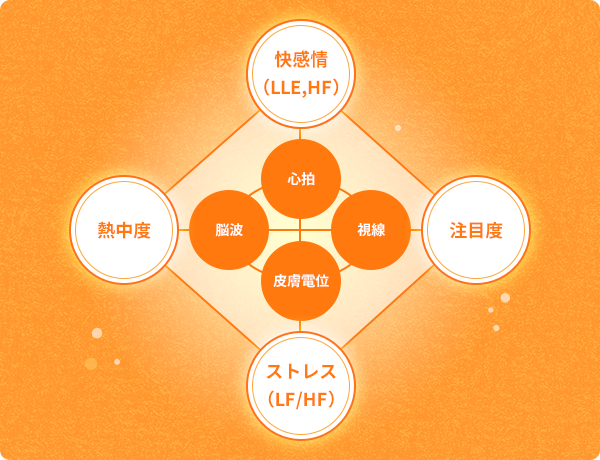
\includegraphics[width=8cm]{images/chapter2/heart.png}
    \caption{生体データからさまざまな感情を取得 : 感情体験メーケティング支援}
    \label{seitaidata}
\end{figure}


\section{生体情報を基にフィードバックする研究}

 生体データを用いて被験者に学習支援をする研究がある\cite{seitai1,seitai2,seitai3}.生体データを使うことでより正確に支援ができるからである.
また生体情報を用いたIotも数多く存在する.生体データを活用してライフケア,ヘルスサービスの実現をしている.
例として図\ref{iot}に示す.生体データを収集することでその人にあった適切なフィードバックが可能である.

\begin{figure}[H]
    \centering
    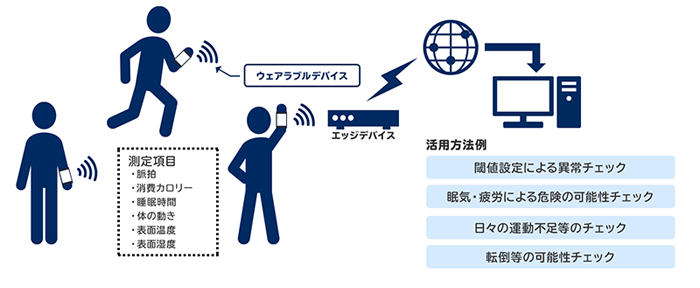
\includegraphics[width=15cm]{images/chapter2/body_img02.png}
    \caption{ウェアラブルデバイスを用いた生体情報のIot : NECソリューションイノベータ}
    \label{iot}
\end{figure}


\section{コンテンツにエフェクトを重畳して面白さを増幅する研究}
コンテンツにエフェクトを重畳して面白さを増幅する研究について述べる。
視線検出装 置を用いてユーザがディスプレイ上の画像において任意の点に注目した際に, 奥行きにフォーカスされた 画像を映像に随時反映し奥行き感を強化する手法が提案されている\cite{shamo1}\cite{shamo2} .
しかし、提案システムはあらかじめ用意した最大 256 枚からなる画像を利用しており, 手軽にコンテンツの視聴体験を拡張, 増幅できるとは言い難いため\cite{shamo3},本研究はエフェクト重畳提示手法を使用した. 

\section{中心視と周辺視の持つ特性の研究}
中心視と周辺視の持つ特性の研究について述べる.
動画コンテンツの周辺にカメラ映像を配置し、動画コンテンツを見ている人の周辺視に何気なく現実世界を提示し,視聴中の動画コンテンツに連動し、
周辺に提示されているカメラ映像に対してエフェクトを付与してカメラ映像内の現実世界を変容させ動画視聴中のユーザの周辺視野を刺激し、動画コンテンツに対する迫力感や恐怖感などを増幅する研究がある\cite{shamo4}.
周辺視では複雑な文字などの図形を部分的にしか認識ができず、中心に近づくほど、より複雑な図形の知覚が可能であり\cite{shamo5},CFF (明滅する光のちらつき感がちょうど消失する周波数)で示される中心視と周辺視の感度差においては、
光のちらつきを最も敏感に感じ取るのは中心ではなく周辺視を明らかにしている\cite{shamo6}.光のちらつきを周辺視がより敏感に感じられるという特性から,周辺視を刺激しコンテンツ視聴体験の拡張を目指し周辺視が人間の知覚能力に及ぼす影響について示している\cite{shamo7}.
周辺視野ほど明るいものがより明るく見え、暗いものはより暗く見える,そして輝度対比効果が強くなる明らかにしているため\cite{shamo8},動画の周辺にエフェクトを提示し,コンテンツに新たな効果を加える.

\section{ユーザの体験を拡張する研究}
ユーザの体験を拡張するという研究について述べる.Focus Plus Context Displayは,高解像度のディスプレイを中心視野用に,低解像度のプロジェクタを周辺視野用にと組み合わせ,低コストで大型ディスプレイを視聴しているのと近い状況を構築する手法を提案している\cite{shamo9}.
また視覚的刺激の提示の有効性はディスプレイ上への提示に限らず,ulumiRoomは,ゲームプレイ時のディスプレイ周辺の壁や床に,プロジェクタからゲームに対応したコンテンツの投影により,臨場感や迫力の増強する手法を実現し\cite{shamo10},
低解像度 LED マトリクスを使用し、適切なオプティカルフローを周辺視に提示をおこない,速度感を提示する手法を実現している\cite{shamo11}.ディスプレイの四周にLED アレイを配置し,ユーザの周辺視野へ動きの提示により,スピード感を増強させるシステムなどを実現し,
LED 点滅パターンの制御をおこない,動きを提示しユーザの感じるスピード感の増強を狙った研究である\cite{shamo12}.本研究は,出力装置を用いず周辺視野を刺激し,動画視聴に新たな効果を加える.
